\section{Basic graph theory}
\subsection{Graph, vertex and edge}
\hspace{\parindent}
A graph G consists of a set of vertices V and a set of edges E, where each edge connects two vertices. Mathematically, we represent a graph as G=(V,E).

A vertex (plural: vertices) is a fundamental unit of a graph, represented as a point. In applications, vertices often represent entities such as people, cities, or computers.

An edge is a connection between two vertices. It can be directed (pointing from one vertex to another) or undirected (bi-directional). Edges often represent relationships or interactions between entities.

\begin{figure}[H]
  \centering
  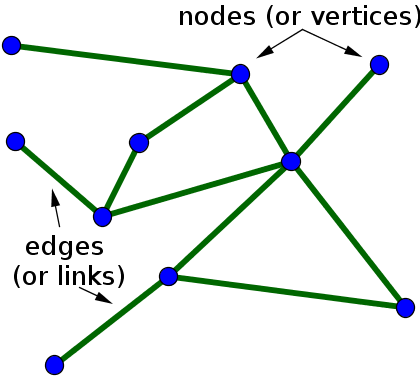
\includegraphics[width=0.4\linewidth]{graph.png}
  \caption{Graph}
  \label{fig:usecase}
\end{figure}

\subsection{Undirected Graph and Directed Graph}
\hspace{\parindent}
A directed graph (or digraph) is a graph where each edge has a direction associated with it. In a directed graph, edges are represented as ordered pairs of vertices.

An undirected graph is a graph where edges do not have any direction associated with them. In an undirected graph, edges are represented as unordered pairs of vertices.

\begin{figure}[H]
  \centering
  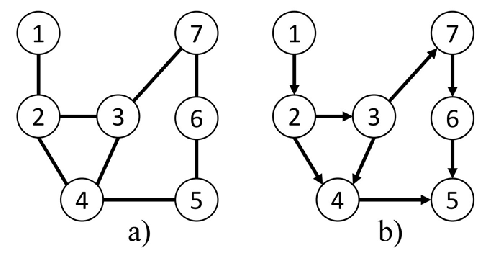
\includegraphics[width=0.4\linewidth]{Undirected-graph-and-b-directed-graph.png}
  \caption{Undirected Graph and Directed Graph}
  \label{fig:usecase}
\end{figure}


\subsection{Degree, path and cycle}
\hspace{\parindent}
The degree of a vertex is the number of edges incident to it. In a directed graph, we can define in-degree (number of incoming edges) and out-degree (number of outgoing edges) for each vertex.

A path in a graph is a sequence of vertices where each adjacent pair of vertices is connected by an edge. The length of a path is the number of edges it contains.

A cycle in a graph is a path that starts and ends at the same vertex, traversing a sequence of distinct vertices and edges.

\section{Graph Neural Network}
\hspace{\parindent}
A GNN is a transformable function applied to all aspects of a graph (including nodes, edges, and global context) while maintaining the graph's symmetries, such as permutation invariance. It represents a subset of deep learning techniques tailored for analyzing data structured as graphs.

These networks are specifically crafted to operate directly on graph data, offering straightforward solutions for tasks involving predictions at the node, edge, or even entire graph levels.

GNNs excel in tasks where Convolutional Neural Networks (CNNs) encounter limitations.

\subsection{Why do Convolutional Neural Networks (CNNs) fail on graphs?}
\hspace{\parindent}

CNNs are highly effective in tasks such as image classification, recognition, or object detection, where they excel in visualizing and analyzing images.

The core principle of CNNs involves employing hidden convolution and pooling layers to detect spatially localized features using receptive fields in kernel form.

\begin{figure}[H]
  \centering
  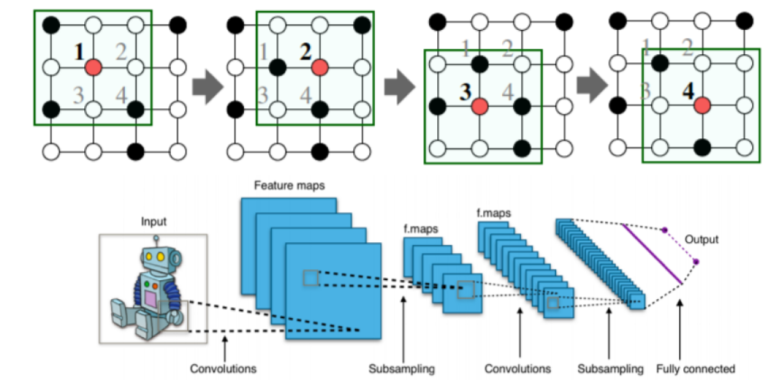
\includegraphics[width=0.7\linewidth]{cnn_on_img.png}
  \caption{CNN}
  \label{fig:usecase}
\end{figure}


Convolution operates on images by sliding a window across a two-dimensional grid, applying a function over each window and passing it through multiple layers.

However, generalizing convolution beyond simple two-dimensional grids poses challenges when applied to graphs due to their arbitrary size and complex topology, lacking spatial locality.

Moreover, the unfixed node ordering in graphs complicates CNN operations, as varying node sequences alter the inputs to the network. Graphs necessitate invariant results regardless of node ordering.


\subsection{The simplest GNN}
\hspace{\parindent}
With the numerical representation of graphs constructed using vectors instead of scalars, the groundwork is laid for building a GNN. The initial step involves constructing the simplest GNN architecture, wherein new embeddings are learned for all graph attributes (nodes, edges, global) without utilizing the graph's connectivity.

This GNN employs separate multilayer perceptrons (MLPs) or another preferred differentiable model for each component of the graph, termed as a GNN layer. For every node vector, the MLP is applied to derive a learned node-vector. This process is repeated for each edge to obtain a per-edge embedding, and similarly for the global-context vector, resulting in a single embedding for the entire graph.

\begin{figure}[H]
  \centering
  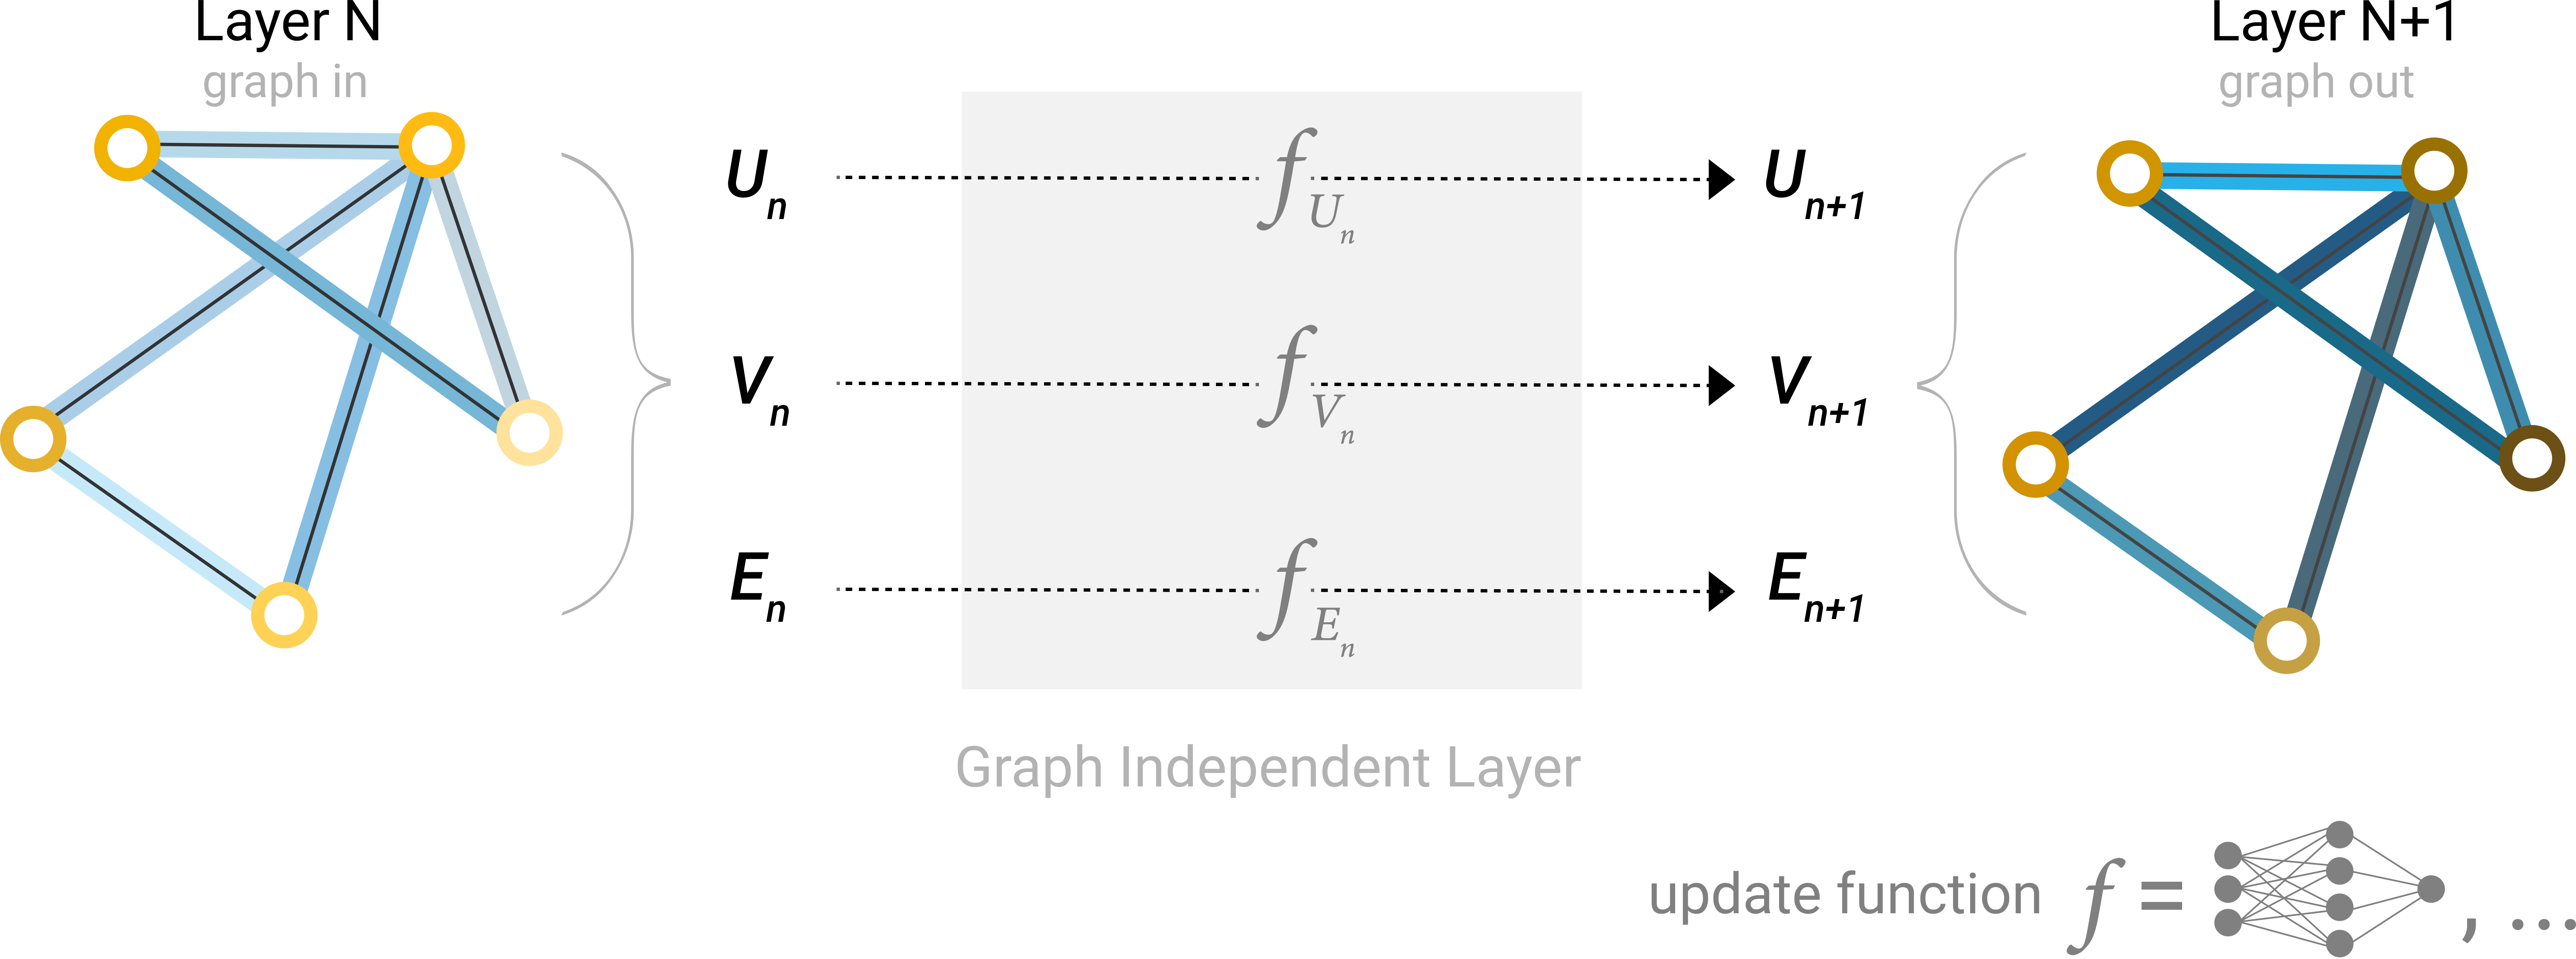
\includegraphics[width=0.7\linewidth]{basis-gnn.png}
  \caption{A basic Graph Neural Network (GNN) consists of a single layer. It takes a graph as input, and each component (V, E, U) is updated by a Multilayer Perceptron (MLP) to generate a new graph. Each function subscript denotes a distinct function corresponding to a different attribute of the graph at the nth layer of the GNN model.}
  \label{fig:usecase}
\end{figure}

As is customary with neural network modules or layers, these GNN layers can be stacked together.

Since a GNN does not alter the connectivity of the input graph, the output graph of a GNN can be described using the same adjacency list and featuring the same number of vectors as the input graph. However, the output graph contains updated embeddings, reflecting the GNN's adjustments to each node, edge, and global-context representation.



\subsection{GNN Predictions by Pooling Information}
\hspace{\parindent}
Considering the scenario of binary classification, the framework can be extended to the multi-class or regression case. If the task involves making binary predictions on nodes, given that the graph already contains node information, the approach is straightforward - for each node embedding, apply a linear classifier.

\begin{figure}[H]
  \centering
  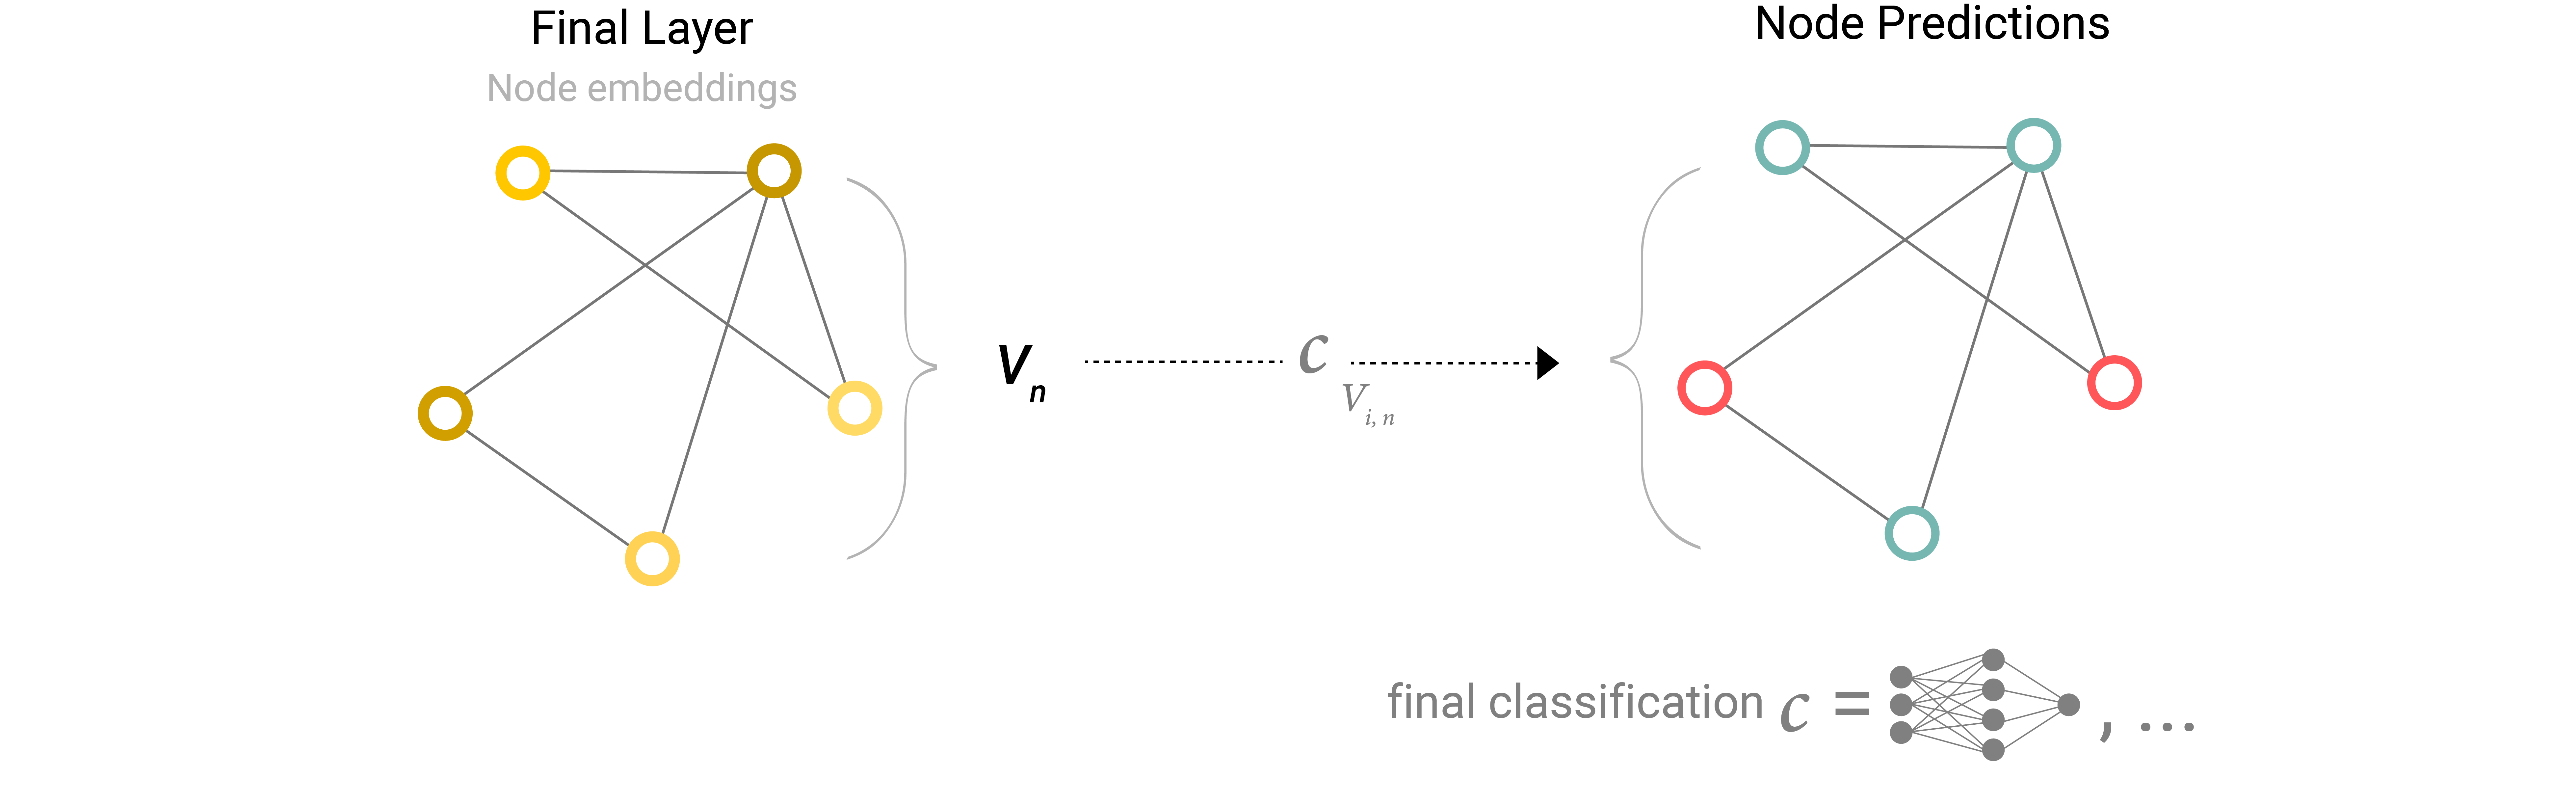
\includegraphics[width=0.7\linewidth]{chap2/2.png}
  \label{fig:usecase}
\end{figure}

However, it's not always straightforward. For instance, information in the graph might be stored in edges but not in nodes, yet predictions on nodes are required. We need a method to gather information from edges and provide it to nodes for prediction. This can be achieved through pooling. Pooling involves two steps.

\begin{enumerate}
    \item For each item to be pooled, gather each of their embeddings and concatenate them into a matrix.
    \item Aggregate the gathered embeddings, usually through a sum operation.
\end{enumerate}

The pooling operation is represented by the letter p, and gathering information from edges to nodes is denoted as pEn->Vn.

\begin{figure}[H]
  \centering
  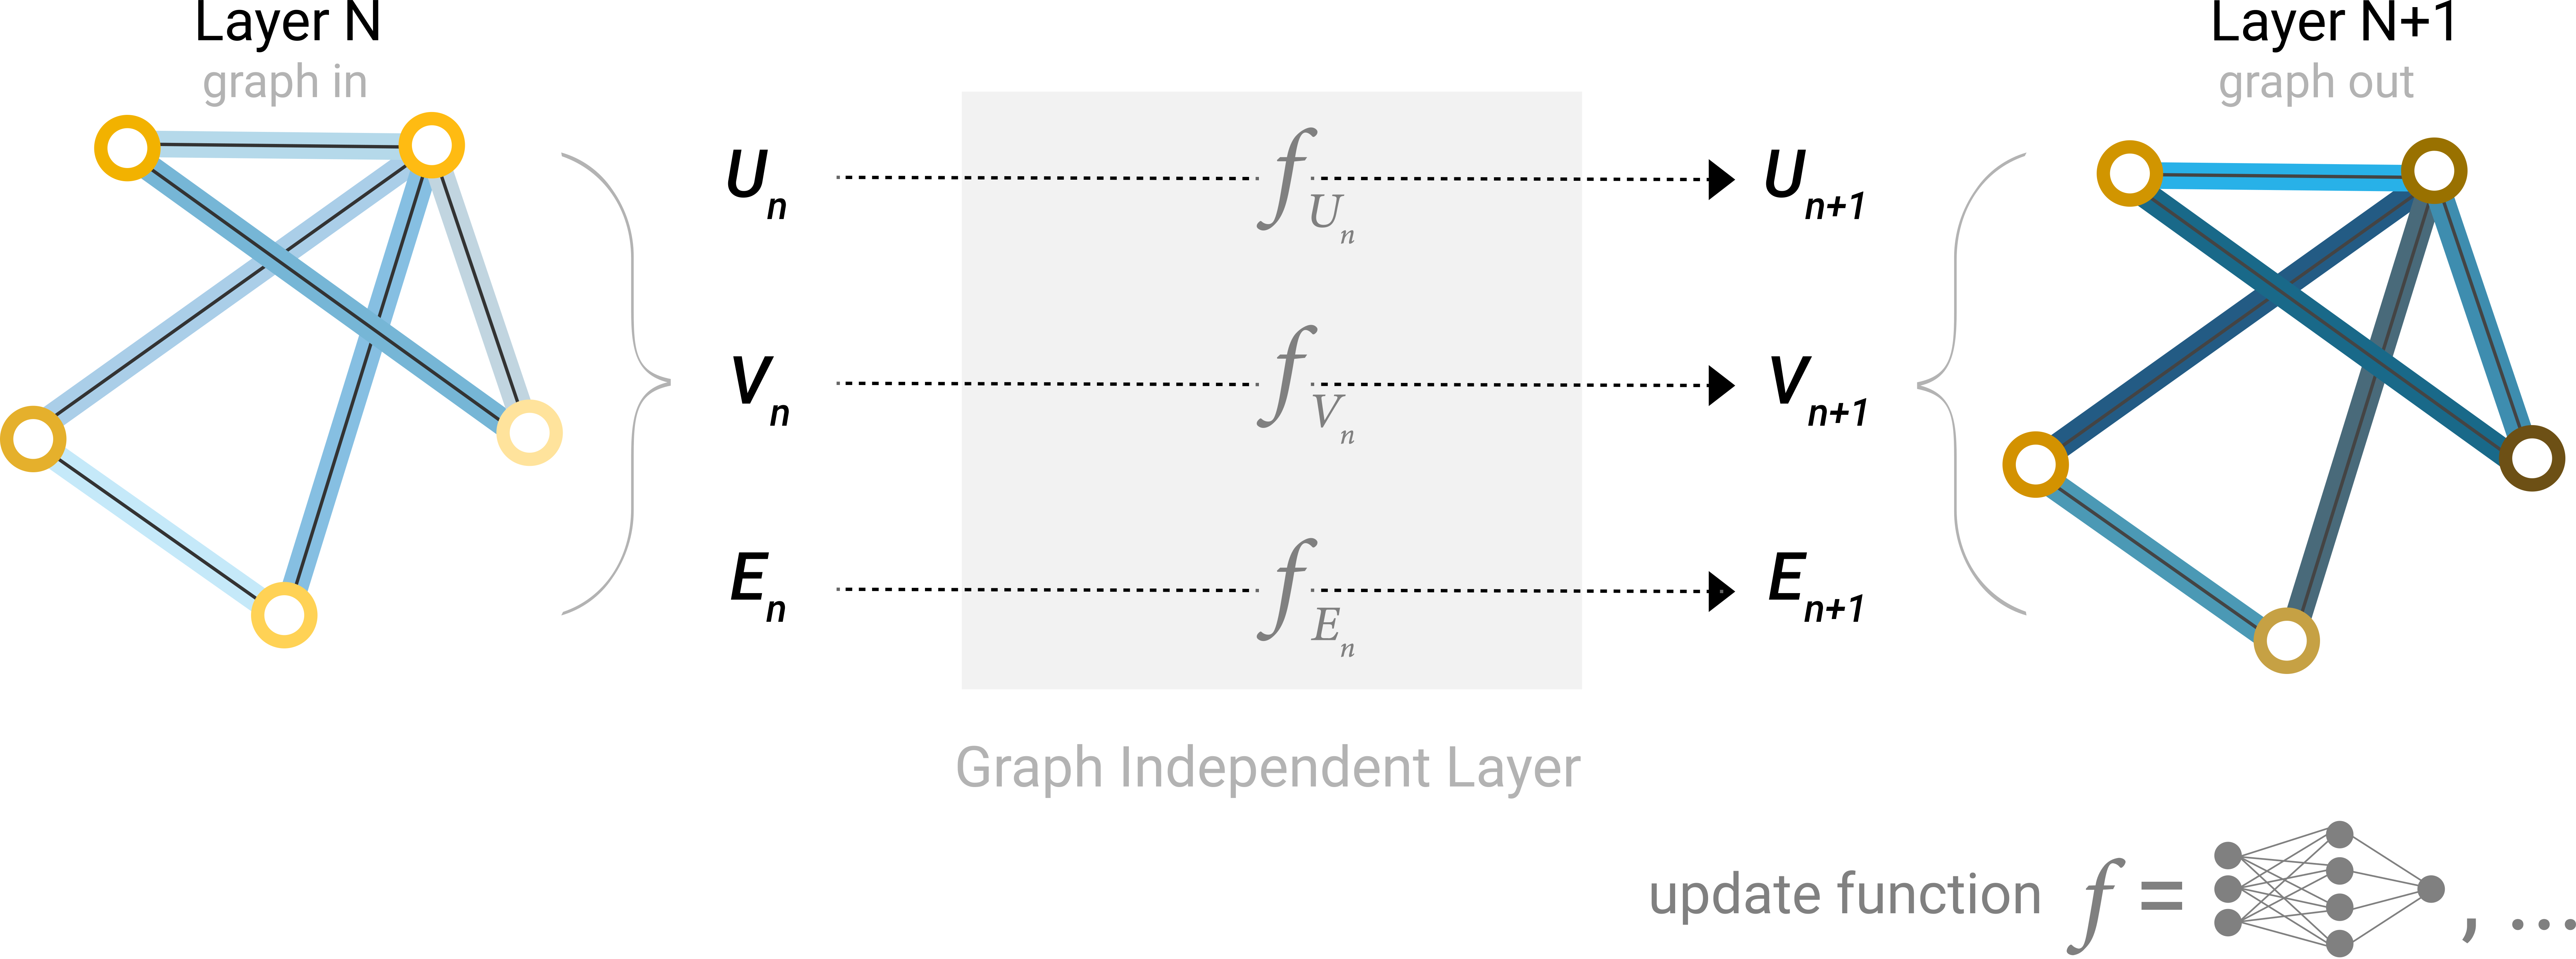
\includegraphics[width=0.7\linewidth]{chap2/3.png}
  \label{fig:usecase}
\end{figure}

So, if only edge-level features are available and the goal is to predict binary node information, pooling can be used to route (or pass) information accordingly. The model resembles this structure.

\begin{figure}[H]
  \centering
  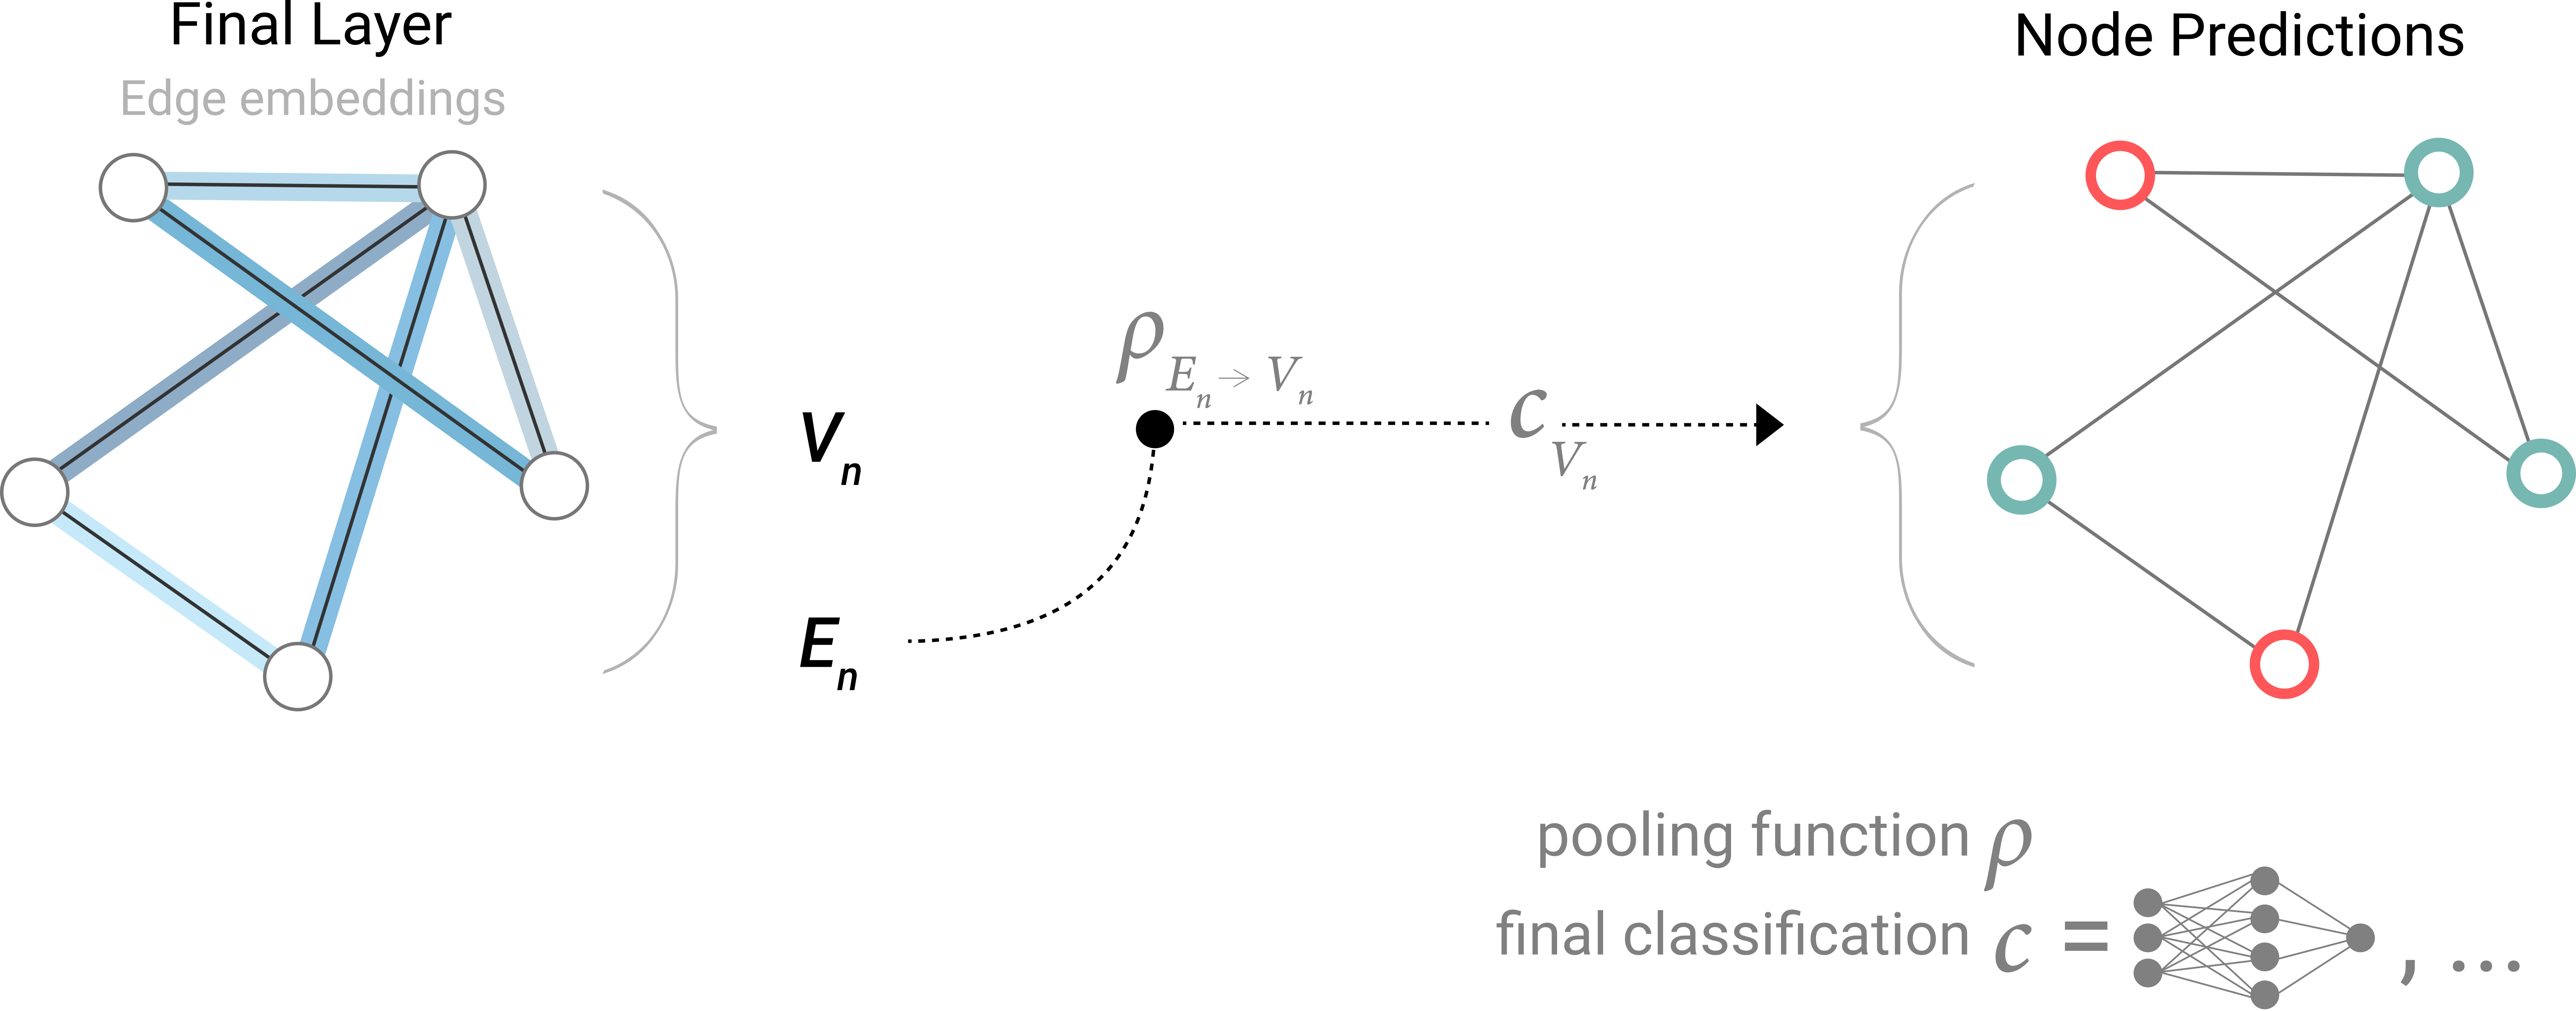
\includegraphics[width=0.7\linewidth]{chap2/4.png}
  \label{fig:usecase}
\end{figure}

Similarly, if only node-level features are available and the objective is to predict binary edge-level information, the model takes a similar form.

\begin{figure}[H]
  \centering
  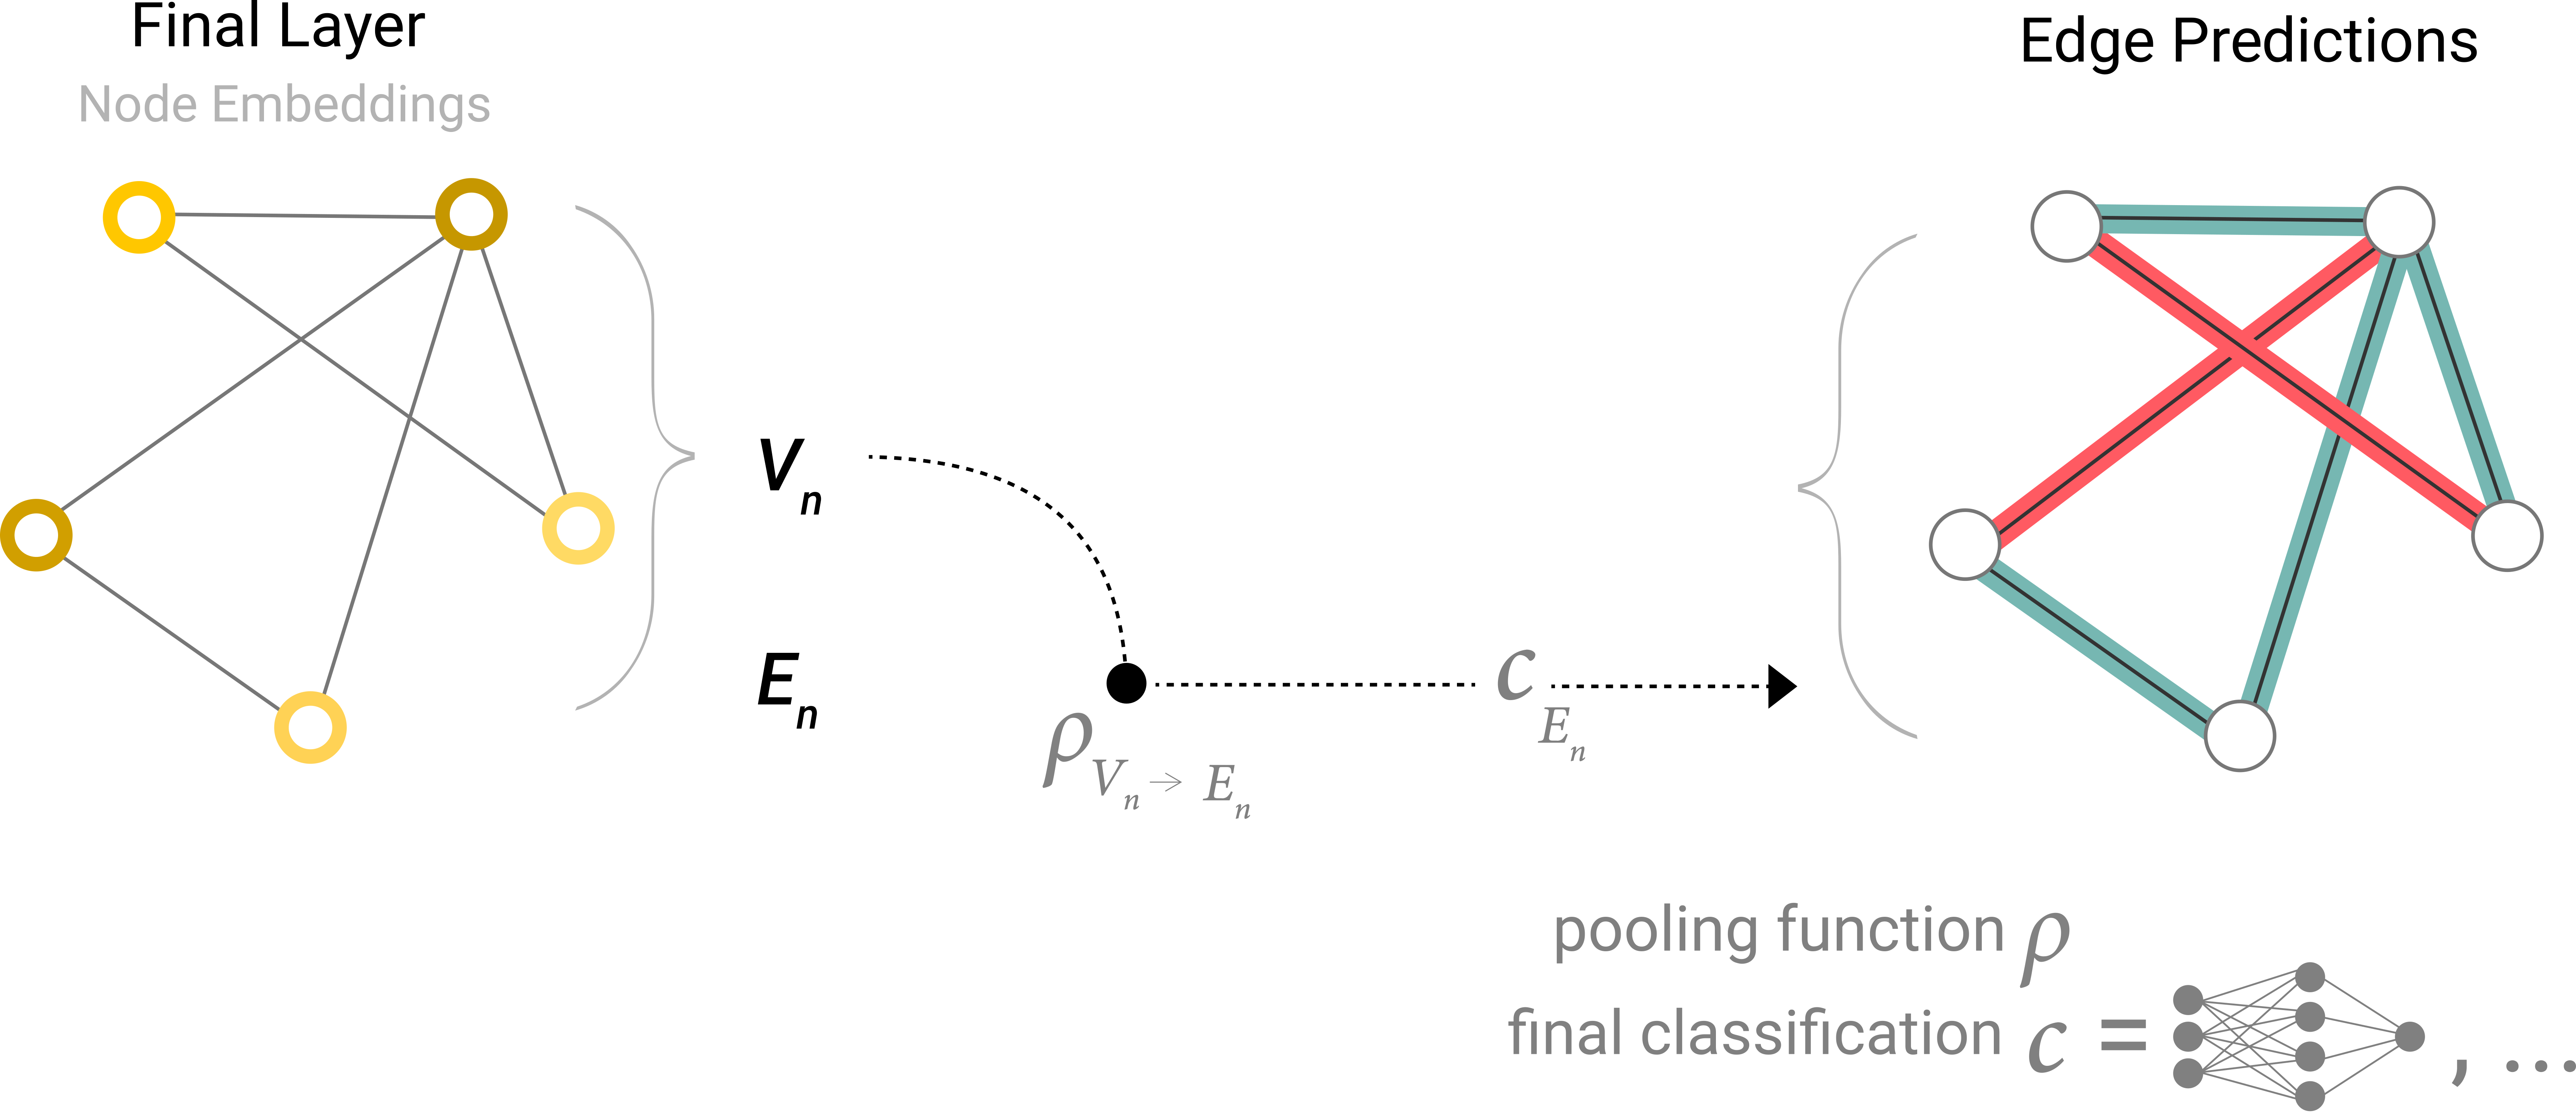
\includegraphics[width=0.7\linewidth]{chap2/5.png}
  \label{fig:usecase}
\end{figure}

When node-level features are available and a binary global property needs to be predicted, all available node information is gathered and aggregated, similar to Global Average Pooling layers in CNNs. The same approach applies to edges.



\begin{figure}[H]
  \centering
  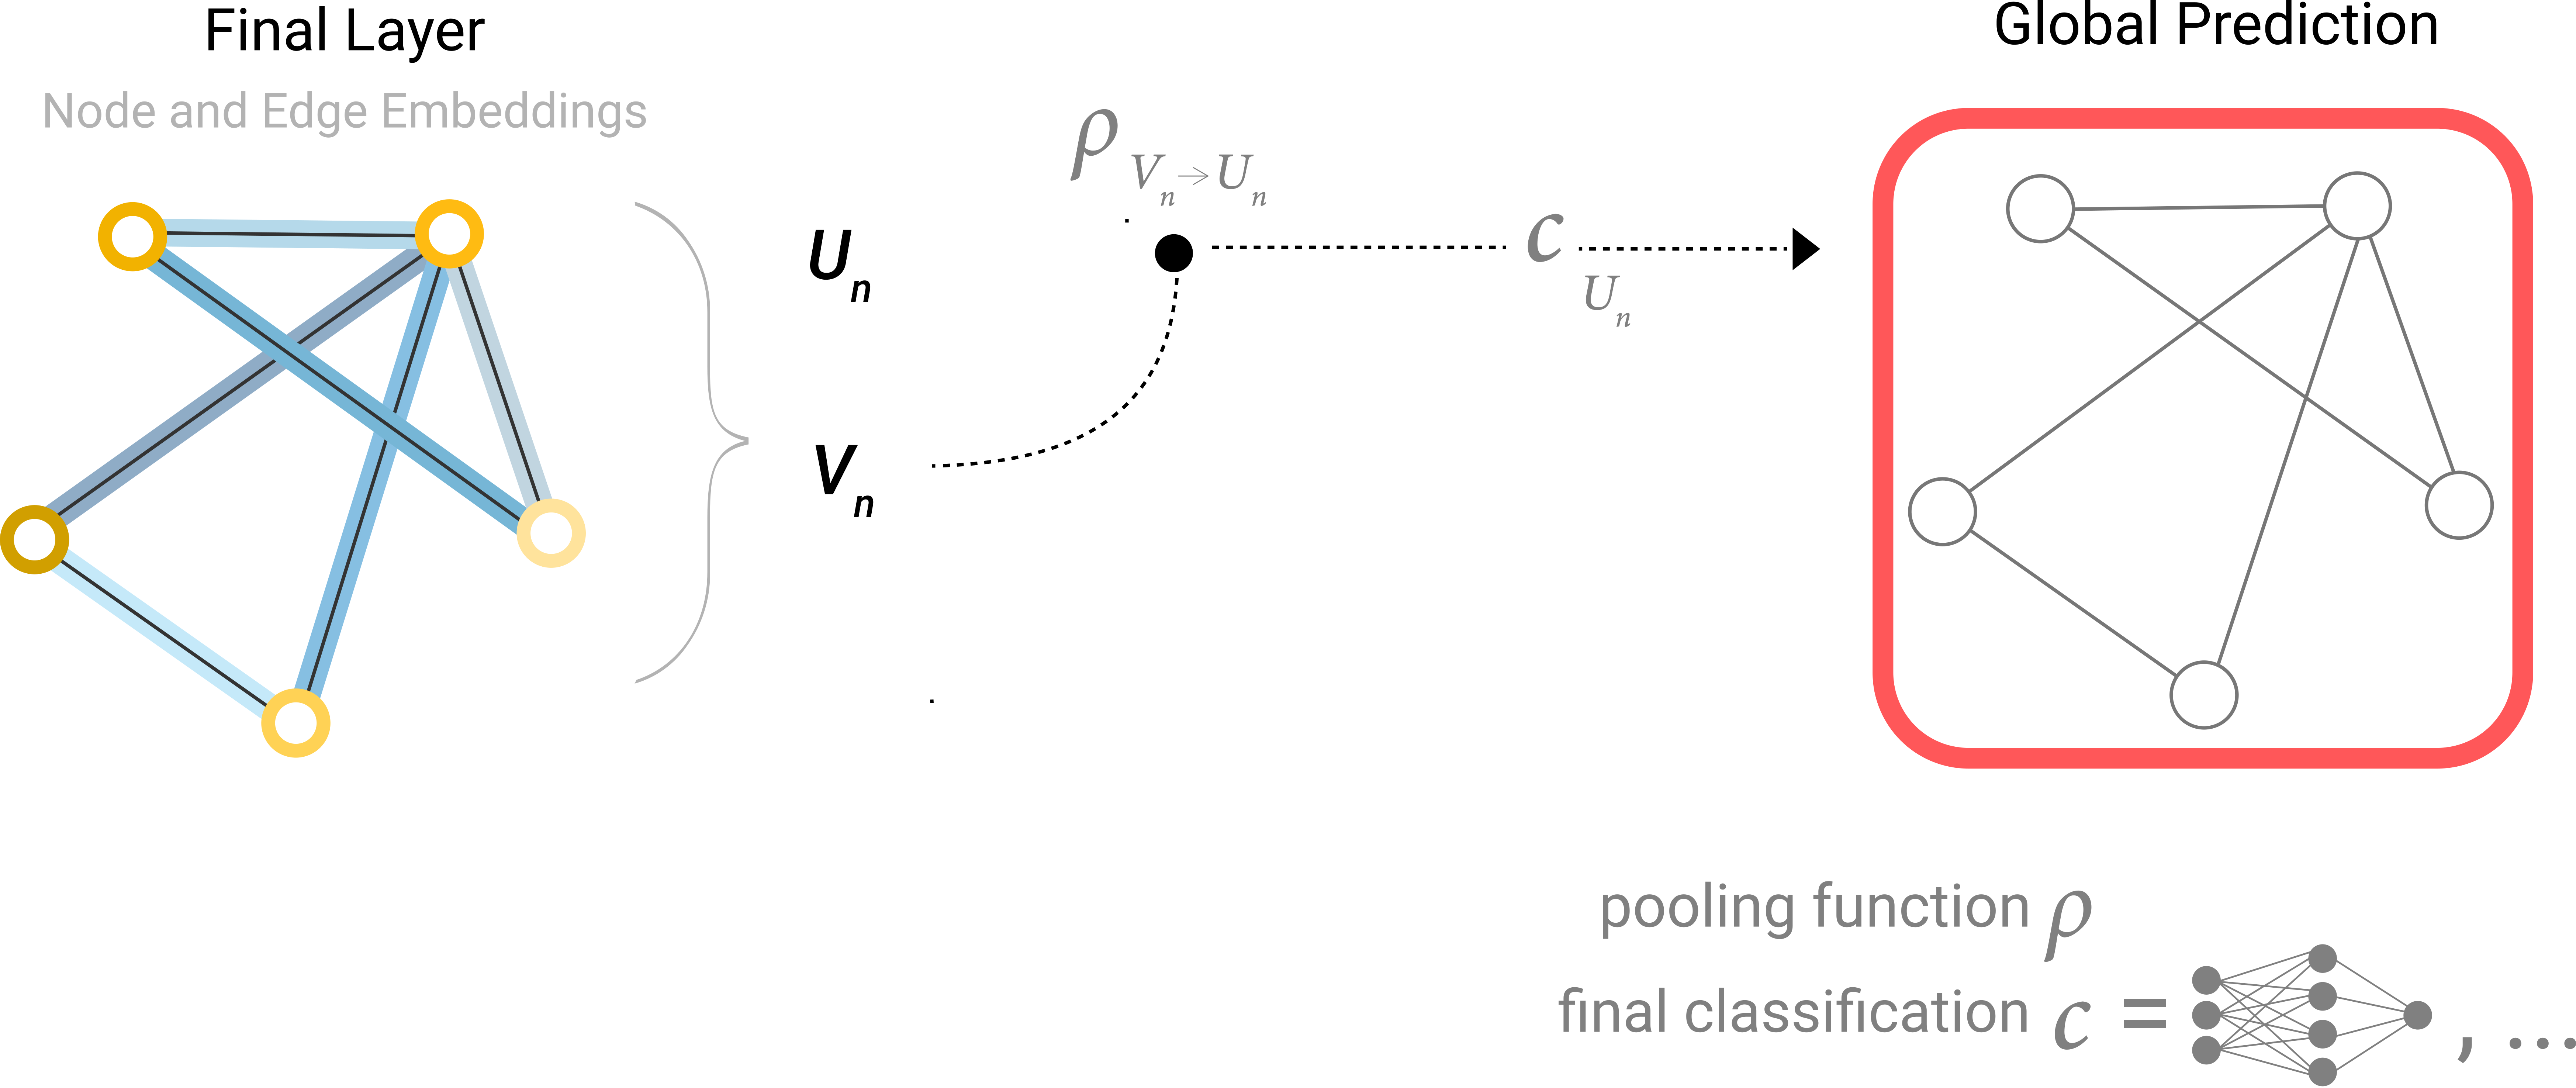
\includegraphics[width=0.7\linewidth]{chap2/6.png}
  \label{fig:usecase}
\end{figure}

In these examples, the classification model c can be replaced with any differentiable model or adapted to multi-class classification using a generalized linear model.


\begin{figure}[H]
  \centering
  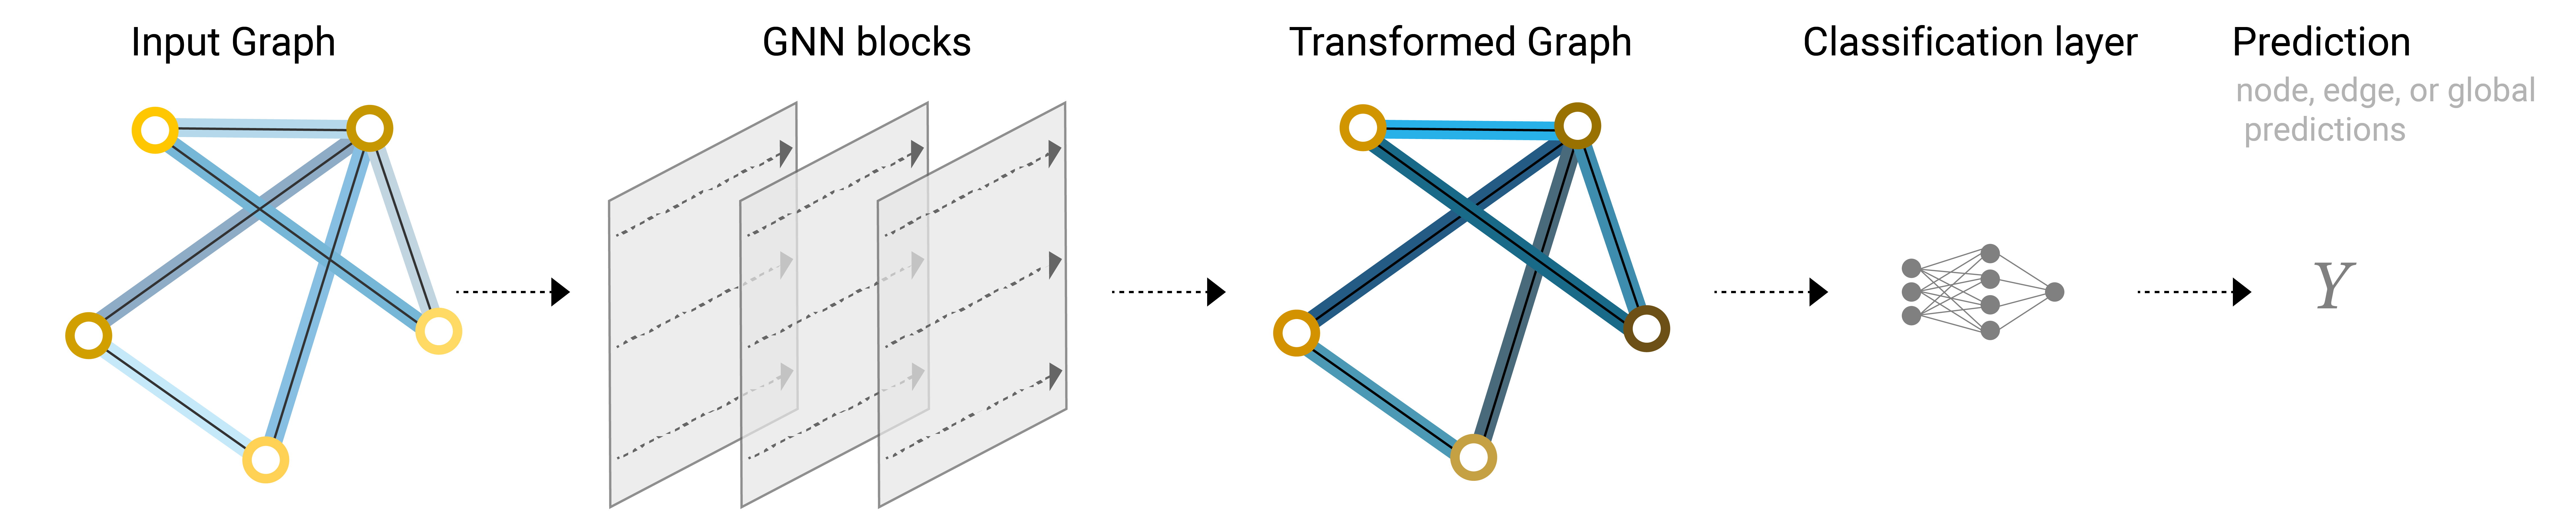
\includegraphics[width=0.7\linewidth]{chap2/7.png}
  \label{fig:usecase}
\end{figure}

Now that a simple GNN model has been demonstrated, and binary predictions can be made by routing information between different parts of the graph, this pooling technique serves as a fundamental building block for constructing more advanced GNN models. If new graph attributes are introduced, defining how to pass information from one attribute to another is all that's required.

It's noteworthy that in this simplest GNN formulation, the connectivity of the graph is not utilized within the GNN layer. Each node, edge, and global context is processed independently, with connectivity only used when pooling information for prediction.







